\documentclass[11pt,a4paper]{article}
\usepackage[T1]{fontenc}
\usepackage[utf8]{inputenc}
\usepackage{lmodern,microtype,amsmath,amssymb,booktabs,graphicx,longtable}
\usepackage[margin=25mm]{geometry}
\usepackage[numbers,sort&compress]{natbib}
\usepackage[colorlinks=true,allcolors=blue]{hyperref}
\hypersetup{pdftitle={Supporting Information: MOUSE Semiempirical Orbital-Optimized DFT},pdfauthor={Vincenzo Barone}}
\usepackage{fancyvrb}
\newcommand{\Eh}{\ensuremath{E_{\rm h}}}
\title{Supporting Information\\Semiempirical Orbital-Optimized DFT in MOUSE:\\Spin-Pure Excited-State Surfaces with Analytic Gradients and Hessians}
\author{Vincenzo Barone}
\date{Working manuscript, 1 November 2026}
\begin{document}
\maketitle
\renewcommand{\thetable}{S\arabic{table}}
\renewcommand{\theequation}{S\arabic{equation}}
\section{Data scope and fixed protocol}
This document preserves separately identified model generations. The early tables describe the relative-active-pair qualification; the final screened symmetry-augmented OO-CID assessment is reported in its own section and table below. Numerical evidence from an earlier model is not attributed to the final candidate. The two parent weights are 0.5, the exchange-response scaling is 0.9, and the additive excitation-energy offset is zero. The full and qualified-spectral parents share their quadratic charge/spin correction and differ in their one-body operator. The mixed-spin and triplet energies within each parent use common spatial orbitals.

The 15 regression states were exposed during development. The four final prospective molecules had previous native/shell-model predictions, but the present full/spectral composite protocol was frozen before their new predictions. Reference transition character, rather than TBE proximity, determines assignments. The reported states constitute a curated qualified cohort; the table is not a survey of every attempted state in preceding development campaigns. In particular, its size must not be used as a database-wide success-rate denominator.

The spectral matching uses occupation-sector assignments with absolute overlap at least 0.7 and a best-versus-alternative margin of at least 0.05. Unqualified orbital levels retain native spacings. There is no fitted orbital-extent correction and no multiplication of the orbital gaps by 0.9. The effective exact-exchange response coefficient is 0.225, and the semilocal response is unchanged. The mean occupied energy sets a gauge for spectral shifts, not a fitted shift of excitation energies.

The two relative active-pair targets are squared cross-parent overlaps at the anchor. They remain fixed while the absolute orbital orientations and spectators relax. Targets within $10^{-10}$ of unity use an exact shared-orbital elimination. The final stationarity certificate concerns the coupled Lagrangian; independent parent orbital gradients are not assumed to vanish away from the anchor. Projected absolute orbital curvatures must exceed $10^{-7}$~\Eh\ for certification. The full-CSF and active-character following thresholds are 0.7.

\clearpage
\section{Complete vertical-energy results}
\begin{table}[!htbp]
\centering\small
\caption{All reported vertical excitation energies and signed errors in eV. The final four rows are prospective tests; the preceding rows are exposed regression examples.}\label{tab:allvertical}
\begin{tabular}{llrrr}
\toprule
Molecule & State & TBE & OO-DFT & Error \\
\midrule
Acetaldehyde & $n\rightarrow\pi^*$ & 4.304 & 4.277 & -0.027 \\
Acetone & $n\rightarrow\pi^*$ & 4.468 & 4.338 & -0.130 \\
Acrolein & $n\rightarrow\pi^*$ & 3.723 & 3.771 & +0.048 \\
Cyclopentadienone & $n\rightarrow\pi^*$ & 2.951 & 2.953 & +0.002 \\
Formamide & $n\rightarrow\pi^*$ & 5.644 & 5.648 & +0.004 \\
Glyoxal & $n\rightarrow\pi^*$ & 2.877 & 2.752 & -0.125 \\
Maleimide & $n\rightarrow\pi^*$ & 3.810 & 3.643 & -0.167 \\
Nitrosomethane & $n\rightarrow\pi^*$ & 1.952 & 1.721 & -0.231 \\
Nitroxyl & $n\rightarrow\pi^*$ & 1.743 & 1.485 & -0.258 \\
Pyranone & $n\rightarrow\pi^*$ & 4.016 & 4.076 & +0.060 \\
Pyrazine & $n\rightarrow\pi^*$ & 4.144 & 3.932 & -0.212 \\
Pyrimidine & $n\rightarrow\pi^*$ & 4.451 & 4.218 & -0.233 \\
Tetrazine & $n\rightarrow\pi^*$ & 2.462 & 2.060 & -0.402 \\
Uracil & $n\rightarrow\pi^*$ & 4.935 & 4.885 & -0.050 \\
Uracil & $\pi\rightarrow\pi^*$ & 5.381 & 5.686 & +0.305 \\
Cyanoformaldehyde & $n\rightarrow\pi^*$ & 3.817 & 3.989 & +0.172 \\
Cyclopropenone & $n\rightarrow\pi^*$ & 4.274 & 4.482 & +0.208 \\
Imidazole & $n\rightarrow\pi^*$ & 6.715 & 6.180 & -0.535 \\
Pyridazine & $n\rightarrow\pi^*$ & 3.830 & 3.530 & -0.300 \\
\bottomrule
\end{tabular}
\end{table}

\section{Direct dedicated sTDA-xTB comparison}
The published dedicated Hamiltonian and parameters are retained. Ground-state xtb4stda wavefunctions and std2 singlet vectors are evaluated at the original XYZs, without geometry optimization or TBE-based root assignment. Cross-basis transition overlaps are normalized only after projection; the norm, overlap, and assignment margin are reported separately in \texttt{data/direct\_stda\_comparison.csv}. All 19 states pass overlap $\geq0.7$, projected norm $\geq0.7$, and margin $\geq0.05$. The small difference between coordinate conversions stored by the legacy executable and the input XYZ is bounded by $2\times10^{-6}$ bohr; no geometry is optimized or refitted. Earlier parameter-path setup failures are preserved separately from the successful electronic attempts.
\begin{longtable}{llrrrrr}
\caption{Every direct sTDA-xTB comparison. Energies and signed errors are in eV; $q$ is the absolute normalized cross-AO transition overlap.}\label{tab:allstda}\\
\toprule Molecule & State & TBE & MOUSE & sTDA-xTB & $\Delta_{\rm sTDA}$ & $q$\\\midrule\endfirsthead
\toprule Molecule & State & TBE & MOUSE & sTDA-xTB & $\Delta_{\rm sTDA}$ & $q$\\\midrule\endhead
Acetaldehyde & $n\pi^*$ & 4.304 & 4.277 & 4.454 & +0.150 & 0.915 \\
Acetone & $n\pi^*$ & 4.468 & 4.338 & 4.531 & +0.063 & 0.930 \\
Acrolein & $n\pi^*$ & 3.723 & 3.771 & 3.826 & +0.103 & 0.918 \\
Cyanoformaldehyde & $n\pi^*$ & 3.817 & 3.989 & 3.911 & +0.094 & 0.900 \\
Cyclopentadienone & $n\pi^*$ & 2.951 & 2.953 & 2.840 & -0.111 & 0.923 \\
Cyclopropenone & $n\pi^*$ & 4.274 & 4.482 & 3.838 & -0.436 & 0.902 \\
Formamide & $n\pi^*$ & 5.644 & 5.648 & 6.039 & +0.395 & 0.853 \\
Glyoxal & $n\pi^*$ & 2.877 & 2.752 & 2.007 & -0.870 & 0.924 \\
Imidazole & $n\pi^*$ & 6.715 & 6.180 & 7.277 & +0.562 & 0.739 \\
Maleimide & $n\pi^*$ & 3.810 & 3.643 & 3.654 & -0.156 & 0.931 \\
Nitrosomethane & $n\pi^*$ & 1.952 & 1.721 & 0.492 & -1.460 & 0.950 \\
Nitroxyl & $n\pi^*$ & 1.743 & 1.485 & 0.237 & -1.506 & 0.955 \\
Pyranone & $n\pi^*$ & 4.016 & 4.076 & 4.710 & +0.694 & 0.913 \\
Pyrazine & $n\pi^*$ & 4.144 & 3.932 & 4.213 & +0.069 & 0.910 \\
Pyridazine & $n\pi^*$ & 3.830 & 3.530 & 3.810 & -0.020 & 0.921 \\
Pyrimidine & $n\pi^*$ & 4.451 & 4.218 & 4.684 & +0.233 & 0.932 \\
Tetrazine & $n\pi^*$ & 2.462 & 2.060 & 1.753 & -0.709 & 0.946 \\
Uracil & $n\pi^*$ & 4.935 & 4.885 & 5.760 & +0.825 & 0.892 \\
Uracil & $\pi\pi^*$ & 5.381 & 5.686 & 5.210 & -0.171 & 0.884 \\
\bottomrule\end{longtable}

\section{Physical structural accuracy and weight precheck}
The following internal-coordinate references are from the published CCSDR(3)/def2-TZVPP supporting tables (DOI 10.1021/acs.jctc.7b00921): acetaldehyde S19, acetone S20, and maleimide S27. The geometry definitions and reference provenance are retained in \path{data/geometry_reference_comparison.json}. No structural reference was used to fit the energy model.
\begin{longtable}{llrrrr}
\caption{Internal coordinates of MOUSE excited-state minima against CCSDR(3)/def2-TZVPP. These comparisons assess physical accuracy separately from derivative correctness.}\\
\toprule Molecule & Coordinate & MOUSE & Reference & Error & Unit\\\midrule\endfirsthead
\toprule Molecule & Coordinate & MOUSE & Reference & Error & Unit\\\midrule\endhead
Acetaldehyde & C-O & 1.312 & 1.331 & -0.019 & \AA \\
Acetaldehyde & C-C & 1.488 & 1.508 & -0.020 & \AA \\
Acetaldehyde & C-Hald & 1.098 & 1.091 & +0.007 & \AA \\
Acetaldehyde & C-C-O & 116.841 & 115.200 & +1.641 & $^\circ$ \\
Acetaldehyde & C-C-Hald & 113.767 & 119.300 & -5.533 & $^\circ$ \\
Acetaldehyde & pyramidalization & 41.651 & 38.700 & +2.951 & $^\circ$ \\
Acetone & C-O & 1.319 & 1.336 & -0.017 & \AA \\
Acetone & C-C & 1.489 & 1.507 & -0.018 & \AA \\
Acetone & C-C-C & 117.761 & 119.500 & -1.739 & $^\circ$ \\
Acetone & pyramidalization & 30.555 & 42.300 & -11.745 & $^\circ$ \\
Maleimide & N-C & 1.378 & 1.404 & -0.026 & \AA \\
Maleimide & C-O & 1.244 & 1.248 & -0.004 & \AA \\
Maleimide & C-C & 1.426 & 1.432 & -0.006 & \AA \\
Maleimide & C=C & 1.371 & 1.386 & -0.015 & \AA \\
Maleimide & N-H & 1.012 & 1.006 & +0.006 & \AA \\
Maleimide & C-H & 1.072 & 1.074 & -0.002 & \AA \\
Maleimide & C-N-C & 111.090 & 109.800 & +1.290 & $^\circ$ \\
\bottomrule\end{longtable}

\begin{table}[htbp]\centering\small
\caption{Algebraic weight sensitivity for the 19 independently stationary vertical-anchor parent gaps. This is not a test of the weighted off-anchor potential or its Hessian. The production weights remain 0.5/0.5.}
\begin{tabular}{rrrr}\toprule $w_F$ & MAE (eV) & RMSE (eV) & Max. error (eV)\\\midrule
0.00 & 0.210 & 0.257 & 0.645 \\
0.25 & 0.179 & 0.211 & 0.590 \\
0.50 & 0.183 & 0.229 & 0.535 \\
0.75 & 0.239 & 0.300 & 0.583 \\
1.00 & 0.308 & 0.396 & 0.958 \\
\bottomrule\end{tabular}\end{table}

The weight table uses independently stationary vertical parents only. It cannot substitute for reoptimizing a weighted off-anchor coupled problem. The production weight remains 0.5. The separate harmonic nitroxyl precheck is retained in \texttt{data/hno\_harmonic\_comparison.json}; its frequency-order correspondence remains provisional until mode-vector confirmation.

\section{Reference data provenance}
The machine-readable file \texttt{data/tbe\_provenance.json} associates each state with its archived QUEST TBE method. The target basis is aug-cc-pVTZ (AVTZ); AVDZ denotes aug-cc-pVDZ. These are theoretical vertical references, not measured absorption maxima. The full input metadata and inherited state assignments are in \texttt{reference\_provenance.json}. The DFT reference basis is aug-cc-pVDZ; it is distinct from the target basis of the TBE. These values are used for reporting errors, not constructing the semiempirical energy.

\noindent\textbf{Acetaldehyde (n\_pi):} CCSDTQ/AVDZ + [CCSDT/AVTZ - CCSDT/AVDZ].

\noindent\textbf{Acetone (n\_pi):} CCSDTQ/6-31+G(d) + [CC4/AVDZ - CC4/6-31+G(d)] + [CCSDT/AVTZ - CCSDT/AVDZ].

\noindent\textbf{Acrolein (n\_pi):} CCSDTQ/6-31+G(d) + [CC4/AVDZ - CC4/6-31+G(d)] + [CCSDT/AVTZ - CCSDT/AVDZ].

\noindent\textbf{Cyclopentadienone (n\_pi):} CC4/6-31+G(d) + [CCSDT/AVTZ - CCSDT/6-31+G(d)].

\noindent\textbf{Formamide (n\_pi):} CCSDTQ/AVDZ + [CCSDT/AVTZ - CCSDT/AVDZ].

\noindent\textbf{Glyoxal (n\_pi):} CC4/AVDZ + [CCSDT/AVTZ - CCSDT/AVDZ].

\noindent\textbf{Maleimide (n\_pi):} CC4/6-31+G(d) + [CCSDT/AVTZ - CCSDT/AVDZ].

\noindent\textbf{Nitrosomethane (n\_pi):} CCSDTQ/AVDZ + [CCSDT/AVTZ - CCSDT/AVDZ].

\noindent\textbf{Nitroxyl (n\_pi):} CCSDTQP/6-31+G(d) + [CCSDTQ/AVTZ - CCSDTQ/6-31+G(d)].

\noindent\textbf{Pyranone (n\_pi):} CC4/6-31+G(d) + [CCSDT/AVTZ - CCSDT/6-31+G(d)].

\noindent\textbf{Pyrazine (n\_pi):} CC4/6-31+G(d) + [CCSDT/AVTZ - CCSDT/6-31+G(d)].

\noindent\textbf{Pyrimidine (n\_pi):} CC4/6-31+G(d) + [CCSDT/AVTZ - CCSDT/6-31+G(d)].

\noindent\textbf{Tetrazine (n\_pi):} CC4/AVDZ + [CCSDT/AVTZ - CCSDT/AVDZ].

\noindent\textbf{Uracil (n\_pi):} CCSDT/6-31+G(d) + [CC3/AVTZ - CC3/6-31+G(d)].

\noindent\textbf{Uracil (pi\_pi):} CCSDT/6-31+G(d) + [CC3/AVTZ - CC3/6-31+G(d)].

\noindent\textbf{Cyanoformaldehyde (n\_pi):} CC4/AVDZ + [CCSDT/AVTZ - CCSDT/AVDZ].

\noindent\textbf{Cyclopropenone (n\_pi):} CC4/AVDZ + [CCSDT/AVTZ - CCSDT/AVDZ].

\noindent\textbf{Imidazole (n\_pi):} CC4/6-31+G(d) + [CCSDT/AVTZ - CCSDT/6-31+G(d)].

\noindent\textbf{Pyridazine (n\_pi):} CC4/6-31+G(d) + [CCSDT/AVTZ - CCSDT/6-31+G(d)].


\section{Derivative checks and stationarity criteria}
The five nuclear minima satisfy a maximum Cartesian gradient below $3\times10^{-5}$~\Eh/bohr and have positive projected vibrational curvatures. Positive excitation gaps and tracked state character are required as separate checks. Directional checks use central differences of the scalar energy and analytic gradient at $\pm h v$, with $h=2\times10^{-4}$ and $10^{-4}$~bohr. The reported Hessian-vector discrepancy is the largest component of the difference from the analytic Hessian acting on the same direction. No finite differences enter the production gradient or Hessian.

At $h=10^{-4}$~bohr, complete Cartesian-column checks yield:
\begin{center}
\begin{tabular}{lrrr}
\toprule
Molecule & Columns & Maximum Hessian error & Scalar-gradient error\\
\midrule
Nitroxyl & 9 & $1.1512\times10^{-8}$ & $3.6434\times10^{-9}$\\
Formamide & 18 & $4.6669\times10^{-9}$ & $2.2575\times10^{-9}$\\
\bottomrule
\end{tabular}
\end{center}
Hessian errors are in \Eh/bohr$^2$; scalar-gradient errors are in \Eh/bohr. The maximum asymmetry of the numerical Hessians is $8.74\times10^{-9}$ and $5.30\times10^{-9}$~\Eh/bohr$^2$, respectively. Full displacement checks and the two-step directional checks for every minimum are recorded in \texttt{data/SUMMARY.json}. Translational and rotational modes are removed before vibrational stability is assessed. No experimental-frequency accuracy is inferred from these implementation tests.

\clearpage
\section{Optimized geometries and projected harmonic frequencies}
All coordinates below are in Angstrom, in the original atom order. They describe minima of the constrained composite semiempirical surface. The XYZ files are also supplied in \texttt{coordinates/}. These coordinates are not high-level reference geometries.
\par\noindent\begin{minipage}{\linewidth}
\subsection{Acetaldehyde}
\begin{verbatim}
7
acetaldehyde; constrained OO-DFT minimum; coordinates in Angstrom
C   0.2223035093  0.1013277113  0.2334913667
C  -0.9453005961 -0.0251942583 -0.6804940117
O   0.4079243109 -0.8702860896  1.0954507793
H   0.3010447606  1.0841255171  0.7176125575
H  -1.8688390394 -0.3135713164 -0.1481562051
H  -0.7506835894 -0.8350717205 -1.3936582758
H  -1.1076978659  0.9035664200 -1.2182916609
\end{verbatim}
Projected harmonic frequencies (cm$^{-1}$): 186.89, 432.23, 667.85, 973.26, 990.28, 1095.13, 1240.79, 1375.25, 1389.50, 1416.35, 1455.67, 2766.35, 2838.16, 2919.28, 3059.54.

\end{minipage}\par\medskip
\par\noindent\begin{minipage}{\linewidth}
\subsection{Acetone}
\begin{verbatim}
10
acetone; constrained OO-DFT minimum; coordinates in Angstrom
C  -0.5689937111 -0.0533836291 -0.2955897103
C   0.0475047310  1.2845796508 -0.5101289622
C   0.2806363777 -1.2536119814 -0.5275519803
O  -1.8450965398 -0.1685475055 -0.6076164069
H   1.0922037630  1.2729010514 -0.2125706389
H   1.3076035812 -1.0537316303 -0.2352636408
H  -0.0227253198  1.6074367061 -1.5645009174
H  -0.4976868798  2.0329363229  0.0742268604
H   0.2629093176 -1.5736462119 -1.5849234343
H  -0.1140660180 -2.0949327727  0.0514752619
\end{verbatim}
Projected harmonic frequencies (cm$^{-1}$): 148.28, 149.63, 270.71, 368.65, 500.42, 852.57, 968.79, 988.72, 1000.93, 1047.16, 1229.45, 1371.00, 1387.39, 1394.90, 1416.89, 1425.45, 1460.92, 1468.31, 2741.86, 2761.53, 2932.39, 2934.40, 3043.80, 3048.12.

\end{minipage}\par\medskip
\par\noindent\begin{minipage}{\linewidth}
\subsection{Formamide}
\begin{verbatim}
6
formamide; constrained OO-DFT minimum; coordinates in Angstrom
C  -0.1991028844 -0.2725711755  0.5163934339
O   1.0835179824 -0.3792440676  0.1254002010
N  -1.0286807403  0.2161588604 -0.4725654836
H  -0.1480202140  0.3692094734  1.4479826708
H  -0.5794619260  0.4820208966 -1.3402912231
H  -1.8635741275 -0.3394673884 -0.6301074391
\end{verbatim}
Projected harmonic frequencies (cm$^{-1}$): 324.38, 489.56, 567.75, 902.41, 1043.32, 1172.31, 1242.56, 1256.85, 1491.02, 2377.42, 3308.98, 3430.06.

\end{minipage}\par\medskip
\par\noindent\begin{minipage}{\linewidth}
\subsection{Maleimide}
\begin{verbatim}
10
maleimide; constrained OO-DFT minimum; coordinates in Angstrom
C   0.0000000000  1.1364919551  0.0927366553
C   0.0000000000 -1.1364919551  0.0927366554
C  -0.0000000000  0.6854283480 -1.2605427879
C   0.0000000000 -0.6854283480 -1.2605427880
N  -0.0000000000  0.0000000000  0.8725164373
O   0.0000000000  2.2842746107  0.5713837699
O   0.0000000000 -2.2842746107  0.5713837699
H   0.0000000000  0.0000000000  1.8848555803
H  -0.0000000000  1.3571912082 -2.0958657911
H  -0.0000000000 -1.3571912082 -2.0958657910
\end{verbatim}
Projected harmonic frequencies (cm$^{-1}$): 179.17, 288.09, 385.45, 502.10, 527.27, 554.29, 601.09, 618.76, 648.38, 676.37, 705.14, 774.17, 992.59, 1029.27, 1049.28, 1165.93, 1220.57, 1252.23, 1312.02, 1486.37, 1636.37, 3169.72, 3180.16, 3405.90.

\end{minipage}\par\medskip
\par\noindent\begin{minipage}{\linewidth}
\subsection{Nitroxyl}
\begin{verbatim}
3
nitroxyl; constrained OO-DFT minimum; coordinates in Angstrom
O   0.0826117682  0.0000000000  1.1867248604
N  -0.1842703289 -0.0000000000 -0.0200741732
H   0.6016583607 -0.0000000000 -0.6666508772
\end{verbatim}
Projected harmonic frequencies (cm$^{-1}$): 1261.41, 1592.58, 3301.05.

\end{minipage}\par\medskip

\section{Timing interpretation}
Earlier values labelled TDA were built with a symmetrized static response and omitted the nonlocal exchange difference required for the TDA $A$ matrix. Their timing ratios and TDA accuracy claims are withdrawn. The archival measurements are explicitly identified in \path{data/archival_static_response_timing.json}; the corresponding CSV fields are labelled archival static response. Corrected TDA uses the corrected GFN2 ground orbitals, with effective exact exchange 0.225, and agrees with the independent PySCF matrix within $3.6\times10^{-15}$~\Eh.

The batched analytic Jacobian comparison uses the identical retained 44-AO nitropyridine checkpoint and two Oracle threads: 4.13837 versus 0.241612~s, maximum elementwise difference $8.88\times10^{-16}$. This 17.13-fold kernel speedup excludes reference preparation and does not establish an end-to-end advantage. The latest response/ROKS/relative-pair/trial-guard regression suite passes 31 tests on Oracle, including trusted Newton acceleration for resolved soft saddles.

The reduced extension initializes stationary parents from independently assigned NTO and native seeds. It applies local CSF overlap 0.90, attainable single-pair transition fidelity squared above one half, occupied/virtual norms 0.7 and an available-root projected margin of 0.05. The ratio to the leading singular value is a representability diagnostic, not a state probability. Absolute active-orbital anchor overlap is reported diagnostically when a fixed reference transition is supplied. Stationarity and curvature criteria remain unchanged. This assignment amendment is separated from the original 19-state data and from the subsequently locked accuracy assessment. The reduced scope is 14 states in ten molecules, selected after baseline convergence outcomes; no excluded state is silently removed from the original ledger.

\section{Completed reduced extension}
All 14 predictions and matched TDA assignments were locked before label opening. The scope was reduced after inspecting convergence and is not wholly blind. The original prediction lock, scoring output, label-opening record and full scope ledger accompany the document in \path{data/reduced_extension/}. Failed or unresolved earlier attempts remain in the calculation archive.
\begin{longtable}{llrrrrr}
\caption{Every reduced-extension energy (eV). The original prediction lock precedes label opening. TDA uses the corrected GFN2 ground orbitals.}\label{tab:extensionall}\\
\toprule
ID / molecule & Family & TBE & OO & TDA-F & TDA-Q & TDA mean \\
\midrule\endhead
B001 Diazirine & $n\pi^*$ & 4.093 & 4.242 & 5.247 & 4.230 & 4.739 \\
B004 Nitropyridine\_N-oxide & $n\pi^*$ & 4.395 & 4.263 & 4.096 & 4.515 & 4.305 \\
B005 Phthalimide & $n\pi^*$ & 4.186 & 4.070 & 4.029 & 4.004 & 4.016 \\
B007 Adenine & $n\pi^*$ & 5.304 & 4.805 & 4.245 & 5.192 & 4.719 \\
B011 Aza-naphthalene & $n\pi^*$ & 5.346 & 5.279 & 5.054 & 5.507 & 5.281 \\
B014 Adenine & $\pi\pi^*$ & 5.191 & 5.449 & 6.192 & 5.494 & 5.843 \\
B015 Bimane\_Syn & $\pi\pi^*$ & 3.964 & 3.911 & 5.189 & 4.947 & 5.068 \\
B016 Cyclopentadiene & $\pi\pi^*$ & 6.451 & 8.197 & 8.282 & 6.624 & 7.453 \\
B022 Furan & $\pi\pi^*$ & 6.530 & 7.974 & 8.448 & 6.829 & 7.638 \\
B024 Phthalimide & $\pi\pi^*$ & 4.600 & 5.869 & 5.670 & 4.927 & 5.298 \\
B025 Quinoxaline & CT & 6.225 & 6.250 & 5.718 & 5.933 & 5.825 \\
B029 Nitropyridine\_N-oxide & CT & 4.078 & 4.153 & 4.765 & 4.433 & 4.599 \\
B030 Quinoxaline & CT & 4.647 & 5.108 & 6.123 & 4.562 & 5.343 \\
B039 Benzoquinone & Rydberg & 7.083 & 7.681 & 8.582 & 7.212 & 7.897 \\
\bottomrule
\end{longtable}


\section{Complete furan multi-CSF Hessian check}
This check concerns the experimental full-relative-active-frame multi-CSF functional, separately from the original single-CSF minima and derivative checks. All 27 Cartesian columns are included; the maximum error is $2.2852\times10^{-8}$~\Eh/bohr$^2$. Electronic solutions are reoptimized at each displaced point, and all three ground-reference terms are included. Completed points and columns are retained for restart.
\begin{longtable}{rrr}
\caption{Complete 27-column furan total excited-state Hessian validation. Analytic constrained orbital/CI response and all three ground-reference derivatives are included. Central differences reoptimize the state at each displaced geometry with step $2\times10^{-4}$ bohr. Units are $E_h$/bohr for the gradient check and $E_h$/bohr$^2$ for the Hessian.}\label{tab:furancolumns}\\
\toprule
Cartesian column (zero based) & Energy--gradient error & Max. Hessian error \\
\midrule\endfirsthead
\toprule
Cartesian column (zero based) & Energy--gradient error & Max. Hessian error \\
\midrule\endhead
0 & 1.35e-15 & 1.25e-08 \\
1 & 1.63e-09 & 1.65e-08 \\
2 & 8.17e-09 & 1.52e-08 \\
3 & 7.11e-11 & 1.25e-08 \\
4 & 2.07e-09 & 1.65e-08 \\
5 & 8.33e-09 & 1.52e-08 \\
6 & 1.87e-10 & 9.93e-09 \\
7 & 7.82e-09 & 1.83e-08 \\
8 & 6.42e-09 & 2.28e-08 \\
9 & 1.11e-10 & 9.93e-09 \\
10 & 7.84e-09 & 1.83e-08 \\
11 & 6.68e-09 & 2.29e-08 \\
12 & 1.38e-10 & 1.89e-09 \\
13 & 2.22e-11 & 8.80e-09 \\
14 & 3.88e-09 & 2.80e-09 \\
15 & 2.22e-10 & 2.13e-09 \\
16 & 5.37e-09 & 1.16e-08 \\
17 & 2.19e-10 & 2.98e-09 \\
18 & 7.99e-11 & 2.13e-09 \\
19 & 5.20e-09 & 1.16e-08 \\
20 & 1.57e-10 & 2.98e-09 \\
21 & 6.66e-11 & 1.56e-09 \\
22 & 9.31e-10 & 2.77e-09 \\
23 & 3.33e-09 & 9.41e-09 \\
24 & 2.93e-10 & 1.56e-09 \\
25 & 7.62e-10 & 2.78e-09 \\
26 & 3.14e-09 & 9.41e-09 \\
\bottomrule
\end{longtable}


\section{Reproducibility and automatic integration}
The final remote qualification used \texttt{oracle.sns.it}. A transfer audit checked 561 result files and 30 source files; the remote test suite reports 86 passing tests. Cold and resumed executions of the integrated example differ by $1.7764\times10^{-15}$~\Eh. The copied \texttt{data/PROTOCOL.json} identifies the validated source files by SHA256. The source hashes refer to the calculation campaign; the manuscript-generation manifest separately identifies the document inputs and outputs.

The explicit interface selects the following settings:
\begin{Verbatim}[fontsize=\small]
native_excited_method = "roks_50_50"
native_roks_composite_orbital_coupling = "relative_active_pair"
native_roks_composite_following = "character_newton_index"
native_roks_composite_reference_policy = "geometry_only"
native_roks_composite_ground_surface = "native_plus_gaps"
native_roks_composite_component_tracking = "active_pair"
\end{Verbatim}
The example source is \texttt{examples/roks\_relative\_pair.py} in the MOUSE repository. Response paths, two certified seed paths, promotions, and parent saddle indices are supplied explicitly. The accepted generation has precedence over cold seeds. It stores both CSFs, relative targets, multipliers, three restricted ground references, model fingerprints, and the anchor. Defaults for other methods are not changed.

The manuscript-generation script \texttt{build\_assets.py} performs lightweight data aggregation and plotting only. It can be run from the associated MOUSE working tree to regenerate all tables, the validation figure, optimized XYZ files, and TBE method provenance. The accompanying CSV provides all 19 OO-DFT values and explicitly labelled archival static-response controls. The completed reduced-extension corrected TDA and OO values are reported separately below. The four-molecule comparison in the main text is the designated prospective comparison; additional exposed TDA values in the CSV must retain that exposure label.

\section{Public multi-CSF interface qualification}
The explicit research interface is
\begin{Verbatim}[fontsize=\small]
native_excited_method = "multicsf_50_50"
native_multicsf_model_path = Path(".../model.json")
\end{Verbatim}
The model defines promotions, rank, reference transitions and the full relative frame. The example is \path{examples/multicsf_oo_dft.py}. Its input hashes are checked before optimizer-cache access. Accepted generations store both wavefunctions, CI coefficients, three ground references and derivatives; trial evaluations do not publish a new generation. A relocated complete model restores the same accepted state. Checkpoint corruption and modified model arrays are rejected. These checks and 46 distinct regression tests ran on Oracle with two threads. No electronic job ran on the laptop.

The cold full-Hessian interface call takes 98.99~s; restoring the accepted state and its already stored Hessian takes 0.613~s. The latter is not a fresh-Hessian timing. Surface evaluation is instrumented against SCC calls and invokes no DFT/TDA solver. Preparation still requires the archived DFT response and reference transition. All source/result hashes, native-extension hash, logs and portable furan inputs are recorded in the multi-CSF integration qualification archive. The original single-CSF automatic interface above remains a separate model.

The response-only $\lambda$ diagnostic uses 0.85, 0.90 and 0.95, with the one-body DFT reference, semilocal contribution and bare off-diagonal CSF couplings held fixed. Vertical weight and fixed-reference rank perturbations are separate algebraic diagnostics; no new molecular minimum or weighted Hessian is inferred. The actual displaced-reference rank diagnostic is reported below; full F/Q energy recalibration and independent validation remain open.

\section{Symmetry-assigned TD-DFTB and \texorpdfstring{$\Delta$}{Delta}DFTB comparison}
All electronic calculations in this table were already completed on Oracle; the new audit only reads stored wavefunctions, transition weights, occupations and energies. DFTB2 uses mio-1-1 parameters. The auxiliary Gaussian $s/p$ shells define the same angular group representation and are never used to compute an electronic energy or a cross-model radial overlap. Reference axes are reused explicitly to avoid irrep-name changes from equivalent axis conventions. A TD root requires more than 0.999 of the reported transition weight in its assigned irrep. The reference irrep is obtained from its AO transition density, allowing orbital degeneracy and mixing. The $\Delta$DFTB final occupied spin orbitals must have irrep purity above 0.999; their product gives the broken-symmetry determinant's spatial irrep. Only globally first reference singlets are considered for this lowest-state method.

The 19-state TD-DFTB MAE is 0.54547~eV. For the 15 eligible completed $\Delta$DFTB states, its MAE is 0.31353~eV and the same-subset MOUSE MAE is 0.17174~eV. On the four previous prospective cases, TD-DFTB gives 1.05835~eV MAE versus 0.30363~eV for MOUSE; on the three eligible prospective $\Delta$DFTB cases, the respective MAEs are 0.23380 and 0.22655~eV. The original calculations, including unsuccessful SCC attempts for uracil and cyclopentadienone, are retained. No failed calculation is replaced by an assigned energy. Additional bounded Anderson and linear-mixing recoveries retain the same mio-1-1 Hamiltonian, integer occupations and $10^{-10}$ SCC tolerance; both incomplete cases remain unresolved. The backend rejects binary charge restart for this method, so the final recoveries supply the previously converged atomic ground charges through the supported InitialCharges input. All 112 recovery artifacts, including input rejections and unsuccessful SCC histories, are retained separately from the 254 original audit inputs/results. Neither the group-theoretical audit nor the arithmetic score is a cross-model transition-overlap qualification or a new independent validation set.
\begin{longtable}{llrrrr}
\caption{TD-DFTB2 and spin-purified $\Delta$DFTB2 (mio-1-1) on the identical original 19-state geometries. TD assignments use a pure spatial irrep and the within-irrep ordinal of the fixed DFT reference. $\Delta$DFTB is restricted to the first global reference singlet and requires the final broken-symmetry determinant to have the target spatial irrep. These are symmetry/ordinal comparisons without cross-method transition-overlap qualification. All energies are in eV. ``SCC'' denotes an incomplete archived calculation; ``higher'' denotes an inapplicable higher reference state.}\label{tab:dftbsymmetry}\\
\toprule
Molecule & State & TBE & MOUSE & TD-DFTB & $\Delta$DFTB \\
\midrule\endhead
acetaldehyde & $n\pi^*$ & 4.304 & 4.277 & 4.531 & 4.766 \\
acetone & $n\pi^*$ & 4.468 & 4.338 & 4.629 & 4.922 \\
acrolein & $n\pi^*$ & 3.723 & 3.771 & 3.096 & 3.576 \\
cyclopentadienone & $n\pi^*$ & 2.951 & 2.953 & 2.318 & SCC \\
formamide & $n\pi^*$ & 5.644 & 5.648 & 5.651 & 6.002 \\
glyoxal & $n\pi^*$ & 2.877 & 2.752 & 2.346 & 2.621 \\
maleimide & $n\pi^*$ & 3.810 & 3.643 & 2.729 & 3.134 \\
nitrosomethane & $n\pi^*$ & 1.952 & 1.721 & 2.068 & 2.658 \\
nitroxyl & $n\pi^*$ & 1.743 & 1.485 & 1.729 & 2.336 \\
pyranone & $n\pi^*$ & 4.016 & 4.076 & 3.436 & 4.012 \\
pyrazine & $n\pi^*$ & 4.144 & 3.932 & 3.767 & 4.086 \\
pyrimidine & $n\pi^*$ & 4.451 & 4.218 & 4.277 & 4.488 \\
tetrazine & $n\pi^*$ & 2.462 & 2.060 & 2.387 & 2.713 \\
uracil & $n\pi^*$ & 4.935 & 4.885 & 3.809 & SCC \\
uracil & $\pi\pi^*$ & 5.381 & 5.686 & 4.980 & higher \\
cyanoformaldehyde & $n\pi^*$ & 3.817 & 3.989 & 3.946 & 4.274 \\
cyclopropenone & $n\pi^*$ & 4.274 & 4.482 & 3.342 & 4.147 \\
imidazole & $n\pi^*$ & 6.715 & 6.180 & 9.569 & higher \\
pyridazine & $n\pi^*$ & 3.830 & 3.530 & 3.511 & 3.947 \\
\bottomrule
\end{longtable}


\section{Complete cyclopentadiene multi-CSF Hessian check}
All 33 Cartesian columns pass through the public surface, with maximum Hessian error $1.2964\times10^{-7}$~\Eh/bohr$^2$ and maximum energy--gradient difference $9.0270\times10^{-9}$~\Eh/bohr. Accepted anchor and all 66 signed energy/gradient evaluations are retained. A separate lightweight reduction of the transferred checkpoints reproduces every reported error. The cold analytic Hessian call takes 250.27~s, with peak process RSS 878220~KiB; this timing begins after model loading and includes direct state relaxation and all three ground-reference derivative terms. The 66 displaced energy/gradient calls take 465.47~s in total, with median 7.05~s (range 4.07--11.27~s); thus the measured finite-difference Hessian cost is 1.86 times the analytic call for this prepared model. Both timings exclude DFT/model preparation and do not constitute a TDA comparison.

Both furan and cyclopentadiene stored Hessians are symmetric and satisfy the translational acoustic identity and nonstationary rotational-covariance identity $H(\Omega R)=\Omega g$. The largest translation residual is below $2\times10^{-15}$~\Eh/bohr$^2$, the largest rotation residual below $4\times10^{-11}$~\Eh/bohr, and the net torque below $3\times10^{-15}$~\Eh. These identities do not imply a molecular minimum or an experimentally accurate vibrational spectrum.
\begin{longtable}{rrr}
\caption{Complete 33-column cyclopentadiene total-excited-energy Hessian check through the public multi-CSF surface. The fixed rank-two model includes native S0 restoration and both corrected ground subtractions. Each signed displacement is independently reoptimized from the accepted anchor; central step is $2\times10^{-4}$ bohr. Units are $E_h$/bohr and $E_h$/bohr$^2$.}\label{tab:cpdcolumns}\\
\toprule
Cartesian column (zero based) & Energy--gradient error & Max. Hessian error \\
\midrule\endhead
0 & 2.66e-11 & 7.48e-09 \\
1 & 5.33e-11 & 4.07e-09 \\
2 & 1.60e-09 & 1.20e-08 \\
3 & 8.88e-11 & 1.16e-08 \\
4 & 5.02e-09 & 1.89e-08 \\
5 & 9.03e-09 & 1.92e-08 \\
6 & 3.55e-11 & 1.16e-08 \\
7 & 5.03e-09 & 1.89e-08 \\
8 & 8.94e-09 & 1.92e-08 \\
9 & 5.33e-11 & 1.30e-07 \\
10 & 6.93e-09 & 1.58e-08 \\
11 & 5.95e-09 & 2.52e-08 \\
12 & 8.88e-11 & 1.30e-07 \\
13 & 7.13e-09 & 1.58e-08 \\
14 & 5.83e-09 & 2.52e-08 \\
15 & 3.54e-09 & 6.84e-09 \\
16 & 1.78e-10 & 1.52e-09 \\
17 & 8.95e-10 & 4.41e-09 \\
18 & 3.86e-09 & 6.83e-09 \\
19 & 2.00e-10 & 1.52e-09 \\
20 & 1.03e-09 & 4.42e-09 \\
21 & 3.11e-11 & 3.04e-09 \\
22 & 6.71e-09 & 1.88e-08 \\
23 & 4.86e-10 & 2.95e-09 \\
24 & 9.77e-11 & 3.03e-09 \\
25 & 6.63e-09 & 1.88e-08 \\
26 & 5.66e-10 & 2.95e-09 \\
27 & 1.60e-10 & 5.83e-09 \\
28 & 4.23e-10 & 2.99e-09 \\
29 & 3.66e-09 & 1.01e-08 \\
30 & 1.02e-10 & 5.83e-09 \\
31 & 5.43e-10 & 2.99e-09 \\
32 & 3.68e-09 & 1.01e-08 \\
\bottomrule
\end{longtable}


\section{Actual DFT-reference rank and subspace test}
The same three rank-two molecules are recomputed at uniform internal Cartesian scales 0.98 and 1.02 about the geometric center. The state-identity thresholds and nearest-integer effective-pair rule are unchanged. Two same-symmetry singlet roots must converge at residual tolerance $10^{-7}$ Hartree; independently recomputed full-operator residuals certify the final vectors. The final reference solver explicitly restricts the occupied/virtual pair space to the requested irrep, uses two-vector Davidson increments and linear-dependence threshold $10^{-20}$, and saves positive-root Ritz checkpoints. Both previously completed neighboring roots can be transported by exact cross-AO overlap. Forbidden-sector numerical components from earlier full-space restart attempts are rejected; their logs and uncertified vectors remain archived and contribute no accepted result. Completed SCF checkpoints are reused. The six final points and baseline reprojection audit ran on Oracle with Python 3.11.15, NumPy 2.3.5 and PySCF 2.14.0; the native extension hash matches the original integration qualification.

The fresh-native-S0 and transported-original-subspace calculations both retain rank two. Baseline compact transition matrices are reproduced within $5\times10^{-16}$, before the changed references are analyzed. All six target transition overlaps exceed 0.996 and available-competitor margins exceed 0.972. This is a local reference/identity test with exposed data and limited competing-root coverage, not a full F/Q recalibration, a common-target-geometry energy anchoring test, or a new independent benchmark.
\begin{table}[!htbp]
\centering\small
\caption{Actual displaced-reference rank test. PBE0/aug-cc-pVDZ/grid-3 ground states and two same-symmetry TDA roots are recomputed at uniform Cartesian scales 0.98 and 1.02. A fresh restricted native GFN2 S0 defines the compact projection. $N_{\rm pair}$ and rank refer to that normalized compact transition. $f$ is coherent cross-geometry transition overlap with the original fixed DFT root; $p$ is the compact projection norm. This does not recalibrate the complete F/Q energy model.}\label{tab:actualanchorrank}
\begin{tabular}{lrrrrr}
\toprule
Molecule & Scale & $N_{\rm pair}$ & Rank & $f$ & $p$ \\
\midrule
Cyclopentadiene & 0.98 & 1.9927 & 2 & 0.9982 & 0.8256 \\
Cyclopentadiene & 1.02 & 1.9850 & 2 & 0.9985 & 0.8511 \\
Furan & 0.98 & 2.0135 & 2 & 0.9984 & 0.8320 \\
Furan & 1.02 & 2.0071 & 2 & 0.9986 & 0.8585 \\
Phthalimide & 0.98 & 1.5924 & 2 & 0.9962 & 0.9318 \\
Phthalimide & 1.02 & 1.5982 & 2 & 0.9962 & 0.9317 \\
\bottomrule
\end{tabular}
\end{table}


\clearpage
\section{Final frozen cohorts and full-anchor energies}
\begin{table}[!htbp]
\centering\small
\caption{Full F/Q and projected-integral recalibration, evaluated at the original common geometry. The original model definition is reproduced exactly at unit scale. All electronic calculations use Oracle with two threads.}\label{tab:finalanchor}
\begin{tabular}{lrrrr}
\toprule
Molecule & Scale & Gap / eV & Change / eV & Residual / $E_h$ \\
\midrule
Cyclopentadiene & 0.98 & 6.70880 & -0.01134 & 4.5e-15 \\
Cyclopentadiene & 1.02 & 6.72817 & +0.00803 & 5.8e-15 \\
Furan & 0.98 & 6.60398 & -0.06963 & 1.2e-14 \\
Furan & 1.02 & 6.69609 & +0.02248 & 1.3e-14 \\
Phthalimide & 0.98 & 5.18083 & +0.23500 & 6.9e-15 \\
Phthalimide & 1.02 & 5.14244 & +0.19662 & 2.7e-12 \\
\bottomrule
\end{tabular}
\end{table}

\begin{table}[!htbp]
\centering\small
\caption{Frozen primary and subsequent challenges, retained separately by identifier I, C and S. S states share a primary-cohort molecule; they are not new molecular holdouts. Dashes denote no qualified energy, never zero error. $^d$ flags partial double character in the source; $^u$ flags a source reference marked unsafe. Both Criegee states retain the former flag. Errors are against the fixed numerical references.}\label{tab:finalindependent}
\begin{tabular}{lllrrrrr}
\toprule
ID & Molecule & State & Rank & Ref. & OO & $\delta$OO & $\delta$TDA-Q \\
\midrule
I001$^{d}$ & Criegee Intermediate & $^1A''$ & 1 & 2.403 & 2.113 & -0.290 & +0.203 \\
I002$^{d}$ & Criegee Intermediate & $^1A'$ & 1 & 3.715 & 1.851 & -1.864 & +2.676 \\
I003 & Cyclobutadiene & $^1B_{1g}$ & 1 & 3.138 & -- & -- & -- \\
I004 & Benzoxadiazole & $^1B_2$ & 1 & 4.606 & 4.491 & -0.115 & -- \\
I005 & Hexatriene & $^1B_u$ & 1 & 5.341 & 4.912 & -0.429 & -0.022 \\
I006 & Ammonia & $^1A_1$ & 1 & 6.588 & -- & -- & -- \\
C001 & Furofuran & $^1B_u$ & 1 & 5.489 & 5.523 & +0.034 & +0.492 \\
C002 & Furofuran & $^1A_g$ & 1 & 6.027 & 7.067 & +1.040 & +0.231 \\
S001$^{u}$ & Benzoxadiazole & $^1A_1$ & 2 & 4.911 & 4.587 & -0.324 & +0.567 \\
S002 & Benzoxadiazole & $^1A_2$ & 1 & 5.312 & 4.788 & -0.524 & -0.078 \\
S003 & Benzoxadiazole & $^1B_1$ & 1 & 5.840 & 5.489 & -0.351 & -0.029 \\
\bottomrule
\end{tabular}
\end{table}

\clearpage
\section{Furan physical reference and cyclopentadiene descent}
\begin{table}[!htbp]
\centering\small
\caption{Furan internal coordinates versus the same EOM-CCSD stationary-point reference (Table V). Symmetry-equivalent coordinates are averaged.}\label{tab:furanstructure}
\begin{tabular}{lrrrr}
\toprule
Coordinate & EOM-CCSD & MOUSE & Difference & Unit \\
\midrule
O-Calpha & 1.3780 & 1.3812 & +0.0032 & \AA \\
Calpha-Cbeta & 1.4600 & 1.4205 & -0.0395 & \AA \\
Cbeta-Cbeta & 1.4640 & 1.4998 & +0.0358 & \AA \\
Calpha-H & 1.0850 & 1.0683 & -0.0167 & \AA \\
Cbeta-H & 1.0880 & 1.0649 & -0.0231 & \AA \\
Calpha-O-Calpha & 109.600 & 106.833 & -2.767 & deg. \\
O-Calpha-Cbeta & 109.600 & 111.935 & +2.335 & deg. \\
Calpha-Cbeta-Cbeta & 105.600 & 104.648 & -0.952 & deg. \\
O-Calpha-H & 116.600 & 117.039 & +0.439 & deg. \\
Calpha-Cbeta-H & 126.500 & 127.743 & +1.243 & deg. \\
\bottomrule
\end{tabular}
\end{table}

\begin{table}[!htbp]
\centering\small
\caption{Furan symmetric valence A1 stationary-point in-plane frequencies, in cm$^{-1}$. Reference: EOM-CCSD, Gromov et al., DOI 10.1063/1.1578051, Table VI. Correspondence uses symmetry then descending frequency; cross-method mode-vector overlaps are unavailable. The large B2 discrepancy is retained. The five imaginary out-of-plane model modes have no numerical reference entries in that table.}\label{tab:furanphysical}
\begin{tabular}{lrrrr}
\toprule
Irrep & Order & EOM-CCSD & MOUSE & Difference \\
\midrule
A1 & 1 & 3332.0 & 3237.0 & -95.0 \\
A1 & 2 & 3303.0 & 3199.6 & -103.4 \\
A1 & 3 & 1446.0 & 1424.3 & -21.7 \\
A1 & 4 & 1407.0 & 1279.9 & -127.1 \\
A1 & 5 & 1079.0 & 1094.6 & +15.6 \\
A1 & 6 & 1066.0 & 1038.6 & -27.4 \\
A1 & 7 & 974.0 & 971.5 & -2.5 \\
A1 & 8 & 769.0 & 736.2 & -32.8 \\
B2 & 1 & 3451.0 & 3230.3 & -220.7 \\
B2 & 2 & 3305.0 & 3200.2 & -104.8 \\
B2 & 3 & 2914.0 & 1440.1 & -1473.9 \\
B2 & 4 & 1404.0 & 1134.8 & -269.2 \\
B2 & 5 & 1261.0 & 1096.8 & -164.2 \\
B2 & 6 & 1053.0 & 991.1 & -61.9 \\
B2 & 7 & 863.0 & 754.4 & -108.6 \\
\bottomrule
\end{tabular}
\end{table}

The furan reference is the symmetric A1 valence stationary point, not the nonsymmetric minimum. The independent distorted-point energy--gradient check has error $2.46\times10^{-9}$ Hartree/bohr. The cyclopentadiene descendant has 27 positive vibrational frequencies and maximum gradient $2.59\times10^{-5}$ Hartree/bohr. A central gradient difference along the softest cyclopentadiene minimum mode, at $2\times10^{-4}$ bohr, verifies its analytic Hessian action within $1.33\times10^{-10}$ Hartree/bohr$^2$. The retained furan descendant has not reached the same stationarity threshold; no minimum or harmonic spectrum is assigned to it.
\clearpage
\section{Prepared-property cost, memory, and preparation audit}
\begin{table}[!htbp]
\centering\small
\caption{Prepared-property costs on Oracle, two threads. Median wall time over n completed fresh processes (three for small cases, one for the largest three sizes) and maximum whole-process RSS. OO Hessian scope includes energy and total gradient. The three smaller cases use rank one and the three larger cases rank two; size and CSF-rank effects are not separated. Both-parent all-root TDA and a single OO state are different outputs. DFT/FQ preparation and model loading are excluded from the property timer and audited separately.}\label{tab:finalcost}
\begin{tabular}{llrrrrr}
\toprule
Molecule & Property & n & AOs & Rank & Time / s & RSS / MiB \\
\midrule
nitroxyl & tda & 3 & 9 & 1 & 0.014 & 152.3 \\
acetaldehyde & tda & 3 & 16 & 1 & 0.057 & 133.8 \\
acetone & tda & 3 & 22 & 1 & 0.155 & 148.2 \\
Furan & tda & 1 & 24 & 2 & 0.224 & 157.2 \\
Cyclopentadiene & tda & 1 & 26 & 2 & 0.303 & 170.2 \\
Phthalimide & tda & 1 & 49 & 2 & 8.731 & 569.3 \\
nitroxyl & energy & 3 & 9 & 1 & 0.286 & 143.5 \\
acetaldehyde & energy & 3 & 16 & 1 & 0.440 & 153.3 \\
acetone & energy & 3 & 22 & 1 & 0.815 & 164.8 \\
Furan & energy & 1 & 24 & 2 & 0.687 & 179.0 \\
Cyclopentadiene & energy & 1 & 26 & 2 & 0.832 & 199.0 \\
Phthalimide & energy & 1 & 49 & 2 & 11.478 & 1017.1 \\
nitroxyl & gradient & 3 & 9 & 1 & 0.301 & 143.6 \\
acetaldehyde & gradient & 3 & 16 & 1 & 0.374 & 152.9 \\
acetone & gradient & 3 & 22 & 1 & 0.500 & 163.4 \\
Furan & gradient & 1 & 24 & 2 & 0.851 & 197.3 \\
Cyclopentadiene & gradient & 1 & 26 & 2 & 1.042 & 210.8 \\
Phthalimide & gradient & 1 & 49 & 2 & 9.292 & 1035.7 \\
nitroxyl & hessian & 3 & 9 & 1 & 0.684 & 145.0 \\
acetaldehyde & hessian & 3 & 16 & 1 & 1.755 & 163.1 \\
acetone & hessian & 3 & 22 & 1 & 3.460 & 194.1 \\
Furan & hessian & 1 & 24 & 2 & 5.104 & 208.9 \\
Cyclopentadiene & hessian & 1 & 26 & 2 & 7.083 & 235.7 \\
Phthalimide & hessian & 1 & 49 & 2 & 42.224 & 1096.7 \\
\bottomrule
\end{tabular}
\end{table}

\begin{table}[!htbp]
\centering\small
\caption{Available preparation stages for the fresh molecular cohort, in seconds. DFT includes the ground calculation; reference TDA supplies transition identity and rank. F calibration is a separate recorded stage. The final column is worker wall time after lock and imports through prediction closure, not a sum of stages or necessarily cold preparation. Ammonia reuses an earlier DFT checkpoint. Dashes denote unavailable/not executed stages. Historical six-size benchmark preparation totals are unavailable and are not assigned zero.}\label{tab:finalprep}
\begin{tabular}{lrrrrr}
\toprule
Molecule & AOs & DFT & Ref. TDA & F calib. & Worker \\
\midrule
Criegee Intermediate & 14 & 2.20 & 8.31 & 1.52 & 13.66 \\
Cyclobutadiene & 20 & 4.10 & 10.50 & -- & 14.75 \\
Benzoxadiazole & 40 & 38.13 & 73.36 & 77.17 & 249.05 \\
Hexatriene & 32 & 21.37 & 45.07 & 36.35 & 115.60 \\
Ammonia & 7 & 0.51 & 0.88 & -- & 0.99 \\
Furofuran & 36 & 25.57 & 101.69 & 50.16 & 253.83 \\
\bottomrule
\end{tabular}
\end{table}

\clearpage
\section{Complete phthalimide analytic Hessian}
The complete $48\times48$ matrix is obtained with the same Hamiltonian, orbital stationarity and spin-adapted CSF definitions. A first complete profiled evaluation takes 97.08 s. Batched response and reuse of the independent orbital/CI block reproduce that matrix within $1.32\times10^{-12}$ Hartree/bohr$^2$. Along the most negative Cartesian Hessian eigenvector, central differences of relaxed gradients at $2\times10^{-4}$ and $10^{-4}$ bohr have maximum errors $2.7684\times10^{-4}$ and $6.8879\times10^{-5}$ Hartree/bohr$^2$, a ratio of 4.019. Richardson extrapolation gives $4.42\times10^{-7}$ Hartree/bohr$^2$ error. This step-convergence test uses finite differences only for validation; the production Hessian is analytic. The maximum translational identity residual is $5.59\times10^{-15}$ Hartree/bohr$^2$ and the nonstationary rotational-covariance residual is $5.56\times10^{-12}$ Hartree/bohr. Earlier censored timings and all displaced-state checkpoints are retained.
\begin{table}[!htbp]
\centering\small
\caption{Analytic derivative acceleration on the same prepared models: old and current energy-plus-gradient and energy-plus-gradient-plus-Hessian wall times in seconds. Small-case values are medians of three fresh processes; large cases have one. Earlier censored phthalimide timing is retained as a lower bound. Energy models, ranks, weights, scaling and derivative definitions are unchanged.}\label{tab:hessianacceleration}
\begin{tabular}{lrrrr}
\toprule
Molecule & Old E+G & Old E+G+H & New E+G & New E+G+H \\
\midrule
nitroxyl & 0.319 & 0.971 & 0.301 & 0.684 \\
acetaldehyde & 0.867 & 8.493 & 0.374 & 1.755 \\
acetone & 2.063 & 62.848 & 0.500 & 3.460 \\
Furan & 3.308 & 104.156 & 0.851 & 5.104 \\
Cyclopentadiene & 5.248 & 251.653 & 1.042 & 7.083 \\
Phthalimide & 71.118 & $\geq600$ & 9.292 & 42.224 \\
\bottomrule
\end{tabular}
\end{table}


\section{Bounded energy-model diagnostics}
Increasing the furofuran space to fixed rank two gives 5.39274 and 6.86288 eV for the two challenge states, against fixed references 5.489 and 6.027 eV. The corresponding baseline rank-one values are 5.52261 and 7.06733 eV. Thus a larger singles-CSF space only partly reduces the Ag error. A rank-three continuation is closed at its last accepted homotopy checkpoint without assigning an endpoint energy. Fixed-rank manifests explicitly preserve the requested rank instead of reapplying the automatic NTO rank rule.

A separate bounded diagnostic replaces only the F-parent linear reference by the projected converged-DFT-ground Fock operator, preserving all response terms, weights, scaling and zero-offset policy. Its primary-cohort MAE is 0.58854 eV and its two-state furofuran MAE is 0.47656 eV. This construction was frozen before the primary baseline labels were opened; furofuran labels were already exposed. The modest improvement does not establish a universal correction or justify promoting this diagnostic over the frozen baseline. Prediction locks and exposure records are retained separately.
\clearpage
\section{Prospective test of a spin-adapted frontier configuration extension}
The remaining energy-model error motivated a separate research extension of the
orbital-optimized model. This extension is not substituted for the frozen
production model in the preceding tables. Its native GFN2 ground spatial
orbitals are retained, while the reference one-body levels combine the
projected CAM-B3LYP Fock Rayleigh quotients and qualified full-basis orbital
energies with the unchanged weights $1/2,1/2$. The response exchange scale
remains $\lambda=0.9$; orbital gaps are not multiplied by this scale. The
same prepared reference and native spatial orbitals define the TDA control.
The minimum individually matched native-orbital overlap is greater than
$1-10^{-7}$ in every control calculation. Thus the comparison does not use
full-basis DFT spatial orbitals for TDA.

Optimized, ground-orthogonal ROKS singlets and their paired-double
configurations are supplemented by the spin-adapted configurations of
excitation rank at most two in the highest-two-occupied/lowest-two-virtual
space. An auxiliary CSF with absolute overlap at least 0.7 with a retained
CSF is omitted as redundant. The two four-open-shell singlets are exact
$S=0$ Clebsch--Gordan combinations; they are not broken-symmetry determinants
relabeled as singlets. Their same-occupation block is obtained from the
SU(2)-invariant Heisenberg completion of the quadratic spin functional.
Specifically, with singly occupied site densities $D_i$ and feature moments
$q_i$, $M_{ij}=q_i^{\mathsf T}K_s q_j$, the block is the singlet projection of
\begin{equation}
 E_c+\tfrac12\sum_i M_{ii}+4\sum_{i<j}M_{ij}\mathbf S_i\cdot\mathbf S_j.
\end{equation}
This matches every collinear spin diagonal and the two-spin ROKS limit,
without adding a fitted exchange or excitation-energy parameter. Matrix
elements between different occupations use singular-safe Slater--Condon
algebra and the overlap-weighted mean of the diagonal functional residuals.
This is a distinct approximate state-interaction functional, rather than
an exact multi-determinant form of CAM-B3LYP.

The reported excitation energy is the selected full state-interaction
excited eigenvalue minus the independently stationary ground-functional
energy. This is an explicitly state-specific composite reference: the
auxiliary lowest state-interaction eigenvalue is \emph{not} silently reset
to the ground-functional energy. Its additional lowering is recorded
separately and ranges from 0.050 to 2.428 eV in this pilot. Consequently,
these results cannot be interpreted as gaps between eigenvalues of one
balanced ground-and-excited-state Hamiltonian. No scalar excitation offset
is fitted or applied, but this ground-reference approximation remains a
material modeling limitation.

The excitation-rank hierarchy was examined on nine already exposed states.
Rank two was selected after that development analysis; those nine states
are therefore not blind validation. The candidate was then frozen in commit
\texttt{7666f7a} before its acetone and glyoxal predictions. Both molecules
and their labels had appeared in older campaigns, so this is a prospective
new-model check on historically exposed molecules, not a truly blind test.
Across eleven states the MAE is 0.217 eV and the maximum absolute error is
0.552 eV, compared with 1.163 and 3.660 eV for the identical-kernel native-orbital
TDA control. All eleven states meet the fixed wavefunction-assignment gates.
However, the two prospective states alone give MAE 0.385 eV, compared with
0.420 eV for TDA. Glyoxal is underestimated by 0.552 eV; hence the frozen
0.30-eV-MAE/0.50-eV-maximum accuracy gate is not passed. The much larger
improvement on the exposed development set must not be presented as a
universal correction of lone-pair excitations or as an independently
validated advantage over all calibrated TDA models.

\begin{figure}[htbp]\centering
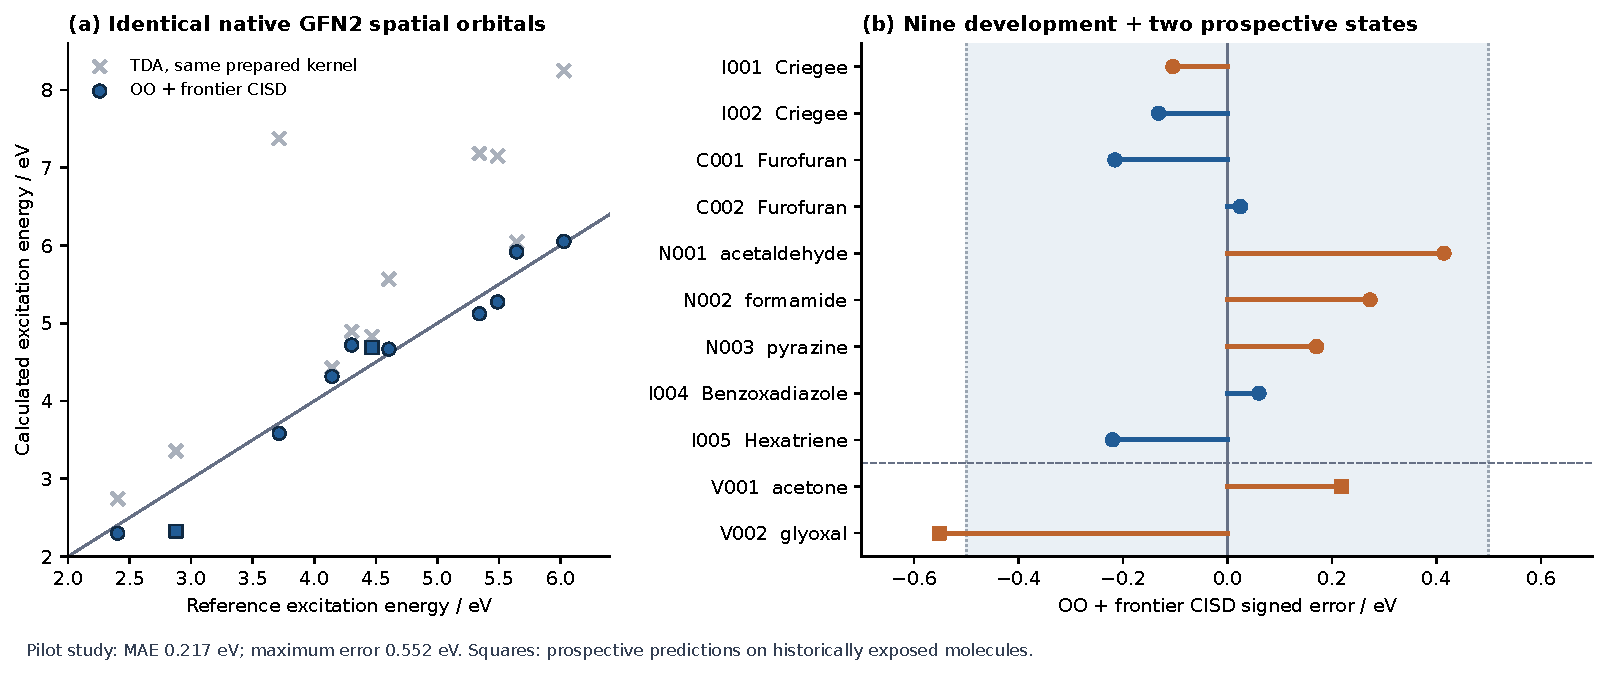
\includegraphics[width=\linewidth]{figures/frontier_cisd_pilot.pdf}
\caption{Exploratory spin-adapted frontier CISD extension. (a) Predictions
and the same-kernel TDA control use the identical native GFN2 ground spatial
orbitals and prepared one-body reference. (b) Signed errors; orange denotes
$n\to\pi^*$ states and blue denotes $\pi\to\pi^*$ states. Squares below the
dashed line identify prospective predictions on historically exposed
molecules. The shaded region is the unchanged $\pm0.5$ eV maximum-error
gate, which glyoxal exceeds.}\label{fig:frontiercisd}
\end{figure}
\begin{table}[htbp]\centering\small
\caption{Pilot vertical excitation energies in eV. The last two rows were
predicted after freezing this candidate.}
\begin{tabular}{llrrr}\hline
ID & Molecule & Reference & OO+CISD & TDA \\ \hline
I001 & Criegee Intermediate & 2.403 & 2.299 & 2.743 \\
I002 & Criegee Intermediate & 3.715 & 3.583 & 7.375 \\
C001 & Furofuran & 5.489 & 5.274 & 7.149 \\
C002 & Furofuran & 6.027 & 6.052 & 8.248 \\
N001 & acetaldehyde & 4.304 & 4.719 & 4.894 \\
N002 & formamide & 5.644 & 5.917 & 6.040 \\
N003 & pyrazine & 4.144 & 4.315 & 4.426 \\
I004 & Benzoxadiazole & 4.606 & 4.666 & 5.565 \\
I005 & Hexatriene & 5.341 & 5.121 & 7.182 \\
V001 & acetone & 4.468 & 4.686 & 4.829 \\
V002 & glyoxal & 2.877 & 2.325 & 3.356 \\
\hline\end{tabular}

\end{table}

The analytic nuclear response is defined for a prepared anchored PES.
Auxiliary canonical orbitals and physical off-diagonal operators are frozen
in the co-rotating orthonormal AO frame; the target ROKS and ground orbitals
retain their complete first and second implicit KKT response. Native diagonal
energies retain explicit geometry and density response. Slater--Condon
matrix elements, overlap metrics, the four-spin block, and the generalized
eigenvalue are differentiated analytically. Auxiliary orbitals are not
re-canonicalized at displaced geometries. This distinction defines the PES
being validated, rather than omitting canonical-orbital response from a
claimed fully re-canonicalized model. Independent displaced, reoptimized
energies are used only to verify the resulting analytic derivatives.

The Criegee target ROKS states can also be recovered from the four canonical
frontier promotions through the ground-program frontend, with no TDA
amplitude reads and no new DFT or SCC call. The exact CSF overlaps with the
retained states differ from unity by less than $10^{-13}$ and the energy
differences are below $4\times10^{-12}$ eV. The corresponding furofuran
recovery has CSF overlaps within $10^{-13}$ of unity and energy differences
below $6\times10^{-12}$ eV. This verifies a TDA-free initialization route
for these four states; it does not establish coverage of CT or Rydberg
states outside the chosen compact orbital space.

Complete analytic Cartesian Hessians of this anchored extension have now
been assembled for both Criegee states (15 coordinates) and both furofuran
states (36 coordinates). Independent reoptimized energies at displacements
of $10^{-3}$ and $5\times10^{-4}$ bohr in two directions verify the
analytic first and second derivatives. Richardson extrapolation of these
validation energies gives maximum gradient errors of $1.12\times10^{-10}$
and $1.31\times10^{-11}$ Hartree/bohr for Criegee and furofuran,
respectively, and directional curvature errors of $1.89\times10^{-7}$ and
$4.03\times10^{-7}$ Hartree/bohr$^2$. The analytic Hessian construction itself
uses no displaced electronic calculation. Raw Hessian asymmetry is at most
$1.16\times10^{-13}$ Hartree/bohr$^2$, and the largest translational sum-rule
residual is $7.20\times10^{-13}$ Hartree/bohr$^2$.

All electronic work for this extension ran on verified Oracle or MAC-STUDIO
hosts. Criegee takes 44.69 s on MAC-STUDIO with two BLAS threads. Furofuran
preserves its already completed sequential columns and completes the remaining
columns with eight independent workers, each using two BLAS threads; that
parallel completion takes 126.83 s. These differently scheduled measurements
are not a common-hardware, common-parallelism scaling benchmark, and the
parallel completion excludes the earlier sequential prefix. They also exclude
one-time DFT-reference preparation. No vertical-energy speed advantage over
TDA is inferred from them.

\clearpage
\section{Earlier compact selected-CID generation (superseded)}
This section preserves the previous model and its qualification. Its two
remaining outliers are resolved by the screened symmetry augmentation
reported in the following final-model section.
The final development step replaces the auxiliary canonical-singles manifold
by a compact selected OO-CID space: the requested optimized, ground-orthogonal
ROKS singlets, their paired doubles, canonical frontier double excitations,
and the two exact four-spin singlets. Unoptimized auxiliary canonical singles
are omitted by excitation rank, using the same rule for every molecule.
This model-space choice was selected using thirteen exposed states. It is
an empirical design choice, not a proof that auxiliary singles always worsen
an orbital-optimized calculation. The common one-body reference averages
Fock Rayleigh quotients and qualified DFT orbital levels \emph{before} orbital
optimization, with weights $1/2,1/2$. This differs from averaging two separately
optimized parent energies. The exchange-response scale remains $\lambda=0.9$.
There is no orbital-gap scaling or fitted excitation offset.

Let $S_{IJ}$ be the CSF metric, $H^0_{IJ}$ the physical Slater--Condon
matrix element, and $d_I=E_I-H^0_{II}/S_{II}$. Away from the exact four-spin
block defined above, the effective matrix is
\begin{equation}
 H_{IJ}=H^0_{IJ}+\tfrac12 S_{IJ}(d_I+d_J).
\end{equation}
The native density functional supplies $E_I$ including spin polarization.
The excited-sector basis is projected orthogonal to the moving stationary
ground CSF $|0\rangle$, using
$|\widetilde I\rangle=|I\rangle-|0\rangle S_{0I}/S_{00}$.
We solve the resulting generalized eigenproblem and subtract the independently
stationary native ground energy. We differentiate this projector as well as
the CSF metric; using an unprojected full-SI root and shifting its energy is
not equivalent. The off-diagonal construction remains an approximate
state-interaction functional; it does not supply a universally balanced
multi-determinant ground-state functional.

The selected rule was frozen in commit \texttt{467a9e5} before evaluating
nitrosomethane and maleimide. The initial fifteen transitions satisfy the unchanged
aggregate MAE gate of 0.3 eV and individual error gate of 0.5 eV, with an MAE
of 0.220 eV and maximum absolute error 0.498 eV. The two post-freeze errors
are $-0.002$ and $+0.402$ eV, respectively, giving 0.202 eV MAE. These
molecules appeared in older campaigns: this is prospective validation of
the frozen candidate on historically exposed molecules, not a blind study.
Glyoxal is within only 0.002 eV of the individual gate; passing that gate
must not be interpreted as a universal correction to all $n\pi^*$ errors.
The same-reference, same-native-orbital TDA control gives 0.966 eV MAE over
these fifteen states. This control isolates the present kernel and is not
a claim to outperform every calibrated TDA or sTDA parameterization.


A further three-molecule cohort was registered in commit \texttt{f8a38e3}
without changing the candidate: pyrimidine tests another diazine substitution
pattern, cyclopentadienone a five-membered conjugated cyclic ketone, and
pyranone a six-membered carbonyl-containing oxygen heterocycle. Their
$n\pi^*$ predictions are 4.637, 3.412 and 4.512 eV, against unchanged
references 4.451, 2.951 and 4.016 eV. All three state assignments pass the
fixed overlap gates and all individual errors remain below 0.5 eV. The
three-state MAE is 0.381 eV, compared with 0.463 eV for the matched native-orbital
TDA control. This subset therefore exceeds the 0.3 eV mean-error criterion;
its successful individual assignments and maximum-error checks must not be
presented as passing every accuracy gate.

Pooling these cases with the original fifteen gave eighteen states in
sixteen molecules, with 0.247 eV MAE and 0.498 eV maximum error. The pooled
mean and maximum meet the original numerical limits, but all five predictions
made after freezing the candidate give 0.309 eV MAE, slightly exceeding the
0.3 eV mean-error limit. These are historically exposed molecules, not a blind
set. The increase from 0.220 to 0.247 eV on extension quantifies the remaining
transferability limitation without modifying the model or its offsets.
The matched TDA control gives 0.882 eV MAE over eighteen states and 0.442 eV
on the five post-freeze predictions. Portable MOUSE evaluation reproduces
all three new matrix predictions without DFT imports, SCC calls or TDA reads;
explicit determinant-sum checks verify $S=0$ for each new state. No additional
nuclear Hessian qualification is claimed for this energy-only extension.
Their archived geometries match the existing Jmol structure plates.


Two final $\pi\pi^*$ targets were registered in commit \texttt{a474e68}:
the $^1A_1$ valence state of furan and the retained uracil target.
The frozen model predicts 5.804 and 6.080 eV, against 6.530 and 5.381 eV,
respectively. Their errors are $-0.726$ and $+0.699$ eV, so both fail the
unchanged 0.5 eV individual-error gate. Coherent state-assignment overlaps
are 0.842 and 0.994, with margins 0.450 and 0.952; numerical convergence
and state assignment pass. Independent portable evaluation reproduces the
same energies with no DFT import, SCC call or TDA read, and explicit
$S^2$ checks confirm pure singlets. This establishes an energy-model
transferability limitation rather than correcting it by numerical convergence.
The opposite deviations are separated by 1.425 eV; no common energy offset
could bring both inside $\pm0.5$ eV. No offset or state-specific rule is applied.

The complete final set contains twenty states in eighteen molecules:
thirteen development states and seven predictions made after freezing the
candidate on historically exposed molecules. Its MAE is 0.293 eV and its
maximum absolute error is 0.726 eV. The seven post-freeze states give
0.425 eV MAE; the two final $\pi\pi^*$ states alone give 0.712 eV MAE.
The pooled mean meets 0.3 eV but the pooled maximum and post-freeze mean
do not meet their original limits. The matched native-orbital TDA control
gives 0.925 eV overall MAE, 0.691 eV on the seven post-freeze states, and
1.313 eV for these last two targets. Improvement relative to this particular
control does not make the final candidate universally accurate. All twenty
predictions, including these two accuracy failures, remain in the figure
and machine-readable table. No new nuclear-derivative claim is added.

\begin{figure}[tbp]\centering
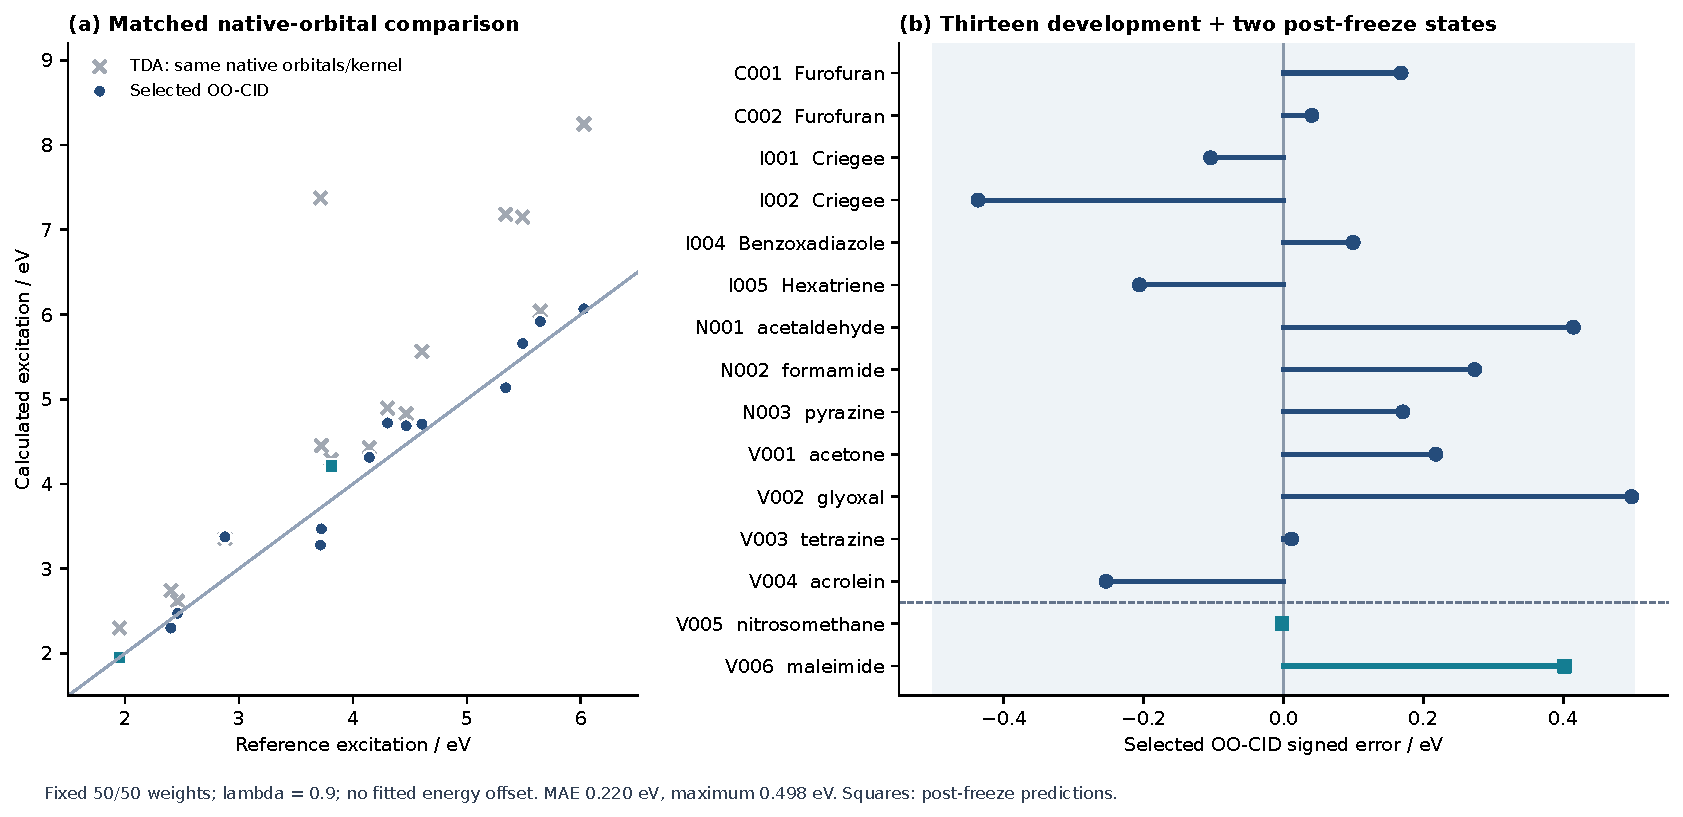
\includegraphics[width=\linewidth]{figures/selected_cid_validation.pdf}
\caption{Final selected OO-CID predictions. The shaded error interval is
$\pm0.5$ eV. Thirteen states informed model selection; squares identify the
seven predictions made after the final candidate freeze. The two last
$\pi\pi^*$ errors lie outside the shaded interval. All controls use
native GFN2 spatial orbitals.}\end{figure}

The public class \texttt{PreparedNOSIModel} evaluates a portable, checksummed
MOUSE surface. LINK selects it with \texttt{nosi\_50\_50}. It uses native ground-program
Fock, energy and derivative machinery, constrained orbital optimization,
and a small CSF eigenproblem. It performs no TDA solve, DFT-backend import,
or fresh ground-state SCC calculation during evaluation. One-time DFT
reference preparation is still required. APOC follows coherent determinant
sums, preserving their phases and checking $\langle S^2\rangle=0$ using
$\|S_+\Psi\|^2$, rather than assigning spin purity to an $M_s=0$ determinant.
Only accepted LINK geometries advance an atomic, model-identified restart;
trial geometries leave that restart unchanged.

Complete analytic Hessians of the final selected model are verified for
Criegee (two states, 15 coordinates), glyoxal (one state, 18 coordinates),
and furofuran (two states, 36 coordinates). Independent reoptimized energy
checks at two displacement sizes and directions validate the first and
second derivatives; these finite differences are validation only. The largest Richardson-extrapolated
errors are $1.33\times10^{-10}$ Hartree/bohr for directional gradients and
$3.28\times10^{-7}$ Hartree/bohr$^2$ for directional curvatures. Both
first and second implicit KKT responses, the moving ground projector,
metric and generalized eigenvector response are retained. Physical operators
and auxiliary orbitals remain fixed in the co-rotating orthonormal AO frame;
this precisely defines an anchored PES, not a re-canonicalized model.
A fresh-process public-API Hessian reproduces the Criegee research matrices
within $9.1\times10^{-13}$ Hartree/bohr$^2$, taking 40.82 s with two BLAS
threads and 262 MiB peak RSS on MAC-STUDIO. Its energy-only evaluation takes
0.135 s. These timings exclude preparation and do not establish a vertical
speed advantage over TDA. The earlier 42.22 s phthalimide Hessian belongs
to the preceding production model, not this final selected candidate.

This completes the finite extension and automatic derivative integration,
while the final $\pi\pi^*$ accuracy failures remain unresolved.
It does not demonstrate an independent broad CT/Rydberg benchmark, final-model
excited minima and frequencies against coupled-cluster theory, or universal
chemical transferability. Those claims require additional evidence beyond
this compact valence-state set.

\begin{table}[htbp]\centering\small\begin{tabular}{llrrr}\toprule
ID & Molecule & Reference & OO-CID & TDA \\ \midrule
C001 & Furofuran & 5.489 & 5.657 & 7.149 \\
C002 & Furofuran & 6.027 & 6.068 & 8.248 \\
I001 & Criegee Intermediate & 2.403 & 2.299 & 2.743 \\
I002 & Criegee Intermediate & 3.715 & 3.278 & 7.375 \\
I004 & Benzoxadiazole & 4.606 & 4.706 & 5.565 \\
I005 & Hexatriene & 5.341 & 5.135 & 7.182 \\
N001 & acetaldehyde & 4.304 & 4.719 & 4.894 \\
N002 & formamide & 5.644 & 5.917 & 6.040 \\
N003 & pyrazine & 4.144 & 4.315 & 4.426 \\
V001 & acetone & 4.468 & 4.686 & 4.829 \\
V002 & glyoxal & 2.877 & 3.375 & 3.356 \\
V003 & tetrazine & 2.462 & 2.473 & 2.616 \\
V004 & acrolein & 3.723 & 3.469 & 4.452 \\
V005 & nitrosomethane & 1.952 & 1.950 & 2.301 \\
V006 & maleimide & 3.810 & 4.212 & 4.286 \\
V007 & pyrimidine & 4.451 & 4.637 & 4.655 \\
V008 & cyclopentadienone & 2.951 & 3.412 & 3.560 \\
V009 & pyranone & 4.016 & 4.512 & 4.591 \\
V010 & Furan & 6.530 & 5.804 & 7.864 \\
V011 & uracil & 5.381 & 6.080 & 6.673 \\
\bottomrule\end{tabular}
\caption{Earlier compact selected OO-CID and same-native-orbital TDA values in eV; this model is superseded by the screened symmetry augmentation.}\end{table}
\clearpage
\section{Selected optimized-target and double-excitation model}
The final development step replaces the auxiliary canonical-singles manifold
by a compact selected OO-CID space: the requested optimized, ground-orthogonal
ROKS singlets, their paired doubles, canonical frontier double excitations,
and the two exact four-spin singlets. Unoptimized auxiliary canonical singles
are omitted by excitation rank, using the same rule for every molecule.
This model-space choice was selected using thirteen exposed states. It is
an empirical design choice, not a proof that auxiliary singles always worsen
an orbital-optimized calculation. The common one-body reference averages
Fock Rayleigh quotients and qualified DFT orbital levels \emph{before} orbital
optimization, with weights $1/2,1/2$. This differs from averaging two separately
optimized parent energies. The exchange-response scale remains $\lambda=0.9$.
There is no orbital-gap scaling or fitted excitation offset.

Let $S_{IJ}$ be the CSF metric, $H^0_{IJ}$ the physical Slater--Condon
matrix element, and $d_I=E_I-H^0_{II}/S_{II}$. Away from the exact four-spin
block defined above, the effective matrix is
\begin{equation}
 H_{IJ}=H^0_{IJ}+\tfrac12 S_{IJ}(d_I+d_J).
\end{equation}
The native density functional supplies $E_I$ including spin polarization.
The excited-sector basis is projected orthogonal to the moving stationary
ground CSF $|0\rangle$, using
$|\widetilde I\rangle=|I\rangle-|0\rangle S_{0I}/S_{00}$.
We solve the resulting generalized eigenproblem and subtract the independently
stationary native ground energy. We differentiate this projector as well as
the CSF metric; using an unprojected full-SI root and shifting its energy is
not equivalent. The off-diagonal construction remains an approximate
state-interaction functional; it does not supply a universally balanced
multi-determinant ground-state functional.

The selected rule was frozen in commit \texttt{467a9e5} before evaluating
nitrosomethane and maleimide. All fifteen transitions satisfy the unchanged
aggregate MAE gate of 0.3 eV and individual error gate of 0.5 eV, with an MAE
of 0.220 eV and maximum absolute error 0.498 eV. The two post-freeze errors
are $-0.002$ and $+0.402$ eV, respectively, giving 0.202 eV MAE. These
molecules appeared in older campaigns: this is prospective validation of
the frozen candidate on historically exposed molecules, not a blind study.
Glyoxal is within only 0.002 eV of the individual gate; passing that gate
must not be interpreted as a universal correction to all $n\pi^*$ errors.
The same-reference, same-native-orbital TDA control gives 0.966 eV MAE over
these fifteen states. This control isolates the present kernel and is not
a claim to outperform every calibrated TDA or sTDA parameterization.

\begin{figure}[tbp]\centering
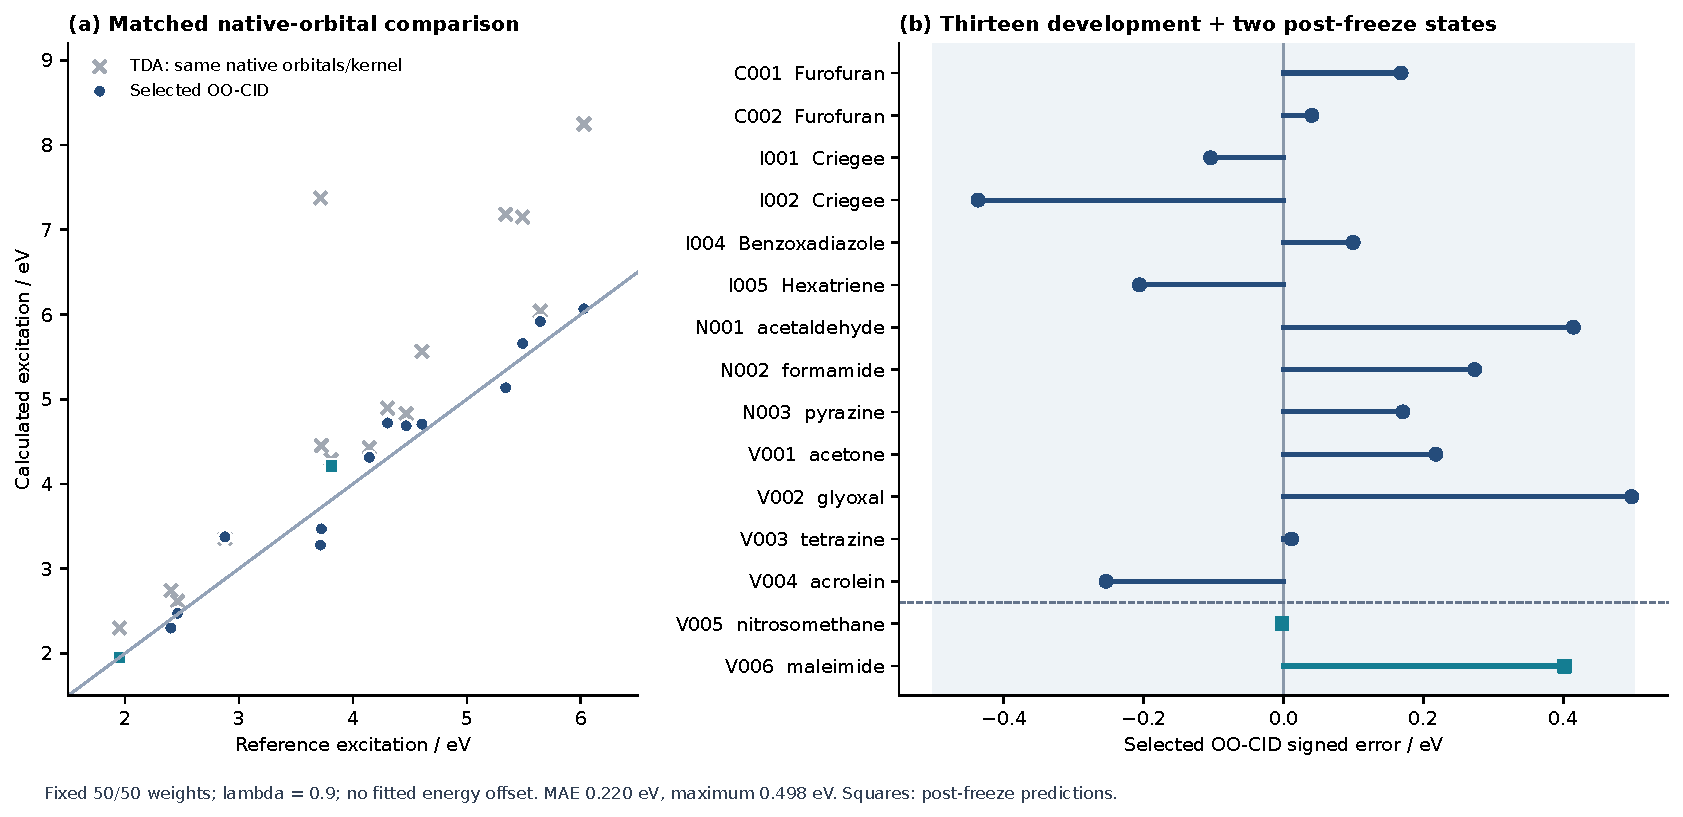
\includegraphics[width=\linewidth]{figures/selected_cid_validation.pdf}
\caption{Final selected OO-CID predictions. The shaded error interval is
$\pm0.5$ eV. Thirteen states informed model selection; squares identify the
two predictions made after the final candidate freeze. All controls use
native GFN2 spatial orbitals.}\end{figure}

The public class \texttt{PreparedNOSIModel} evaluates a portable, checksummed
MOUSE surface. LINK selects it with \texttt{nosi\_50\_50}. It uses native ground-program
Fock, energy and derivative machinery, constrained orbital optimization,
and a small CSF eigenproblem. It performs no TDA solve, DFT-backend import,
or fresh ground-state SCC calculation during evaluation. One-time DFT
reference preparation is still required. APOC follows coherent determinant
sums, preserving their phases and checking $\langle S^2\rangle=0$ using
$\|S_+\Psi\|^2$, rather than assigning spin purity to an $M_s=0$ determinant.
Only accepted LINK geometries advance an atomic, model-identified restart;
trial geometries leave that restart unchanged.

Complete analytic Hessians of the final selected model are verified for
Criegee (two states, 15 coordinates), glyoxal (one state, 18 coordinates),
and furofuran (two states, 36 coordinates). Independent reoptimized energy
checks at two displacement sizes and directions validate the first and
second derivatives; these finite differences are validation only. The largest Richardson-extrapolated
errors are $1.33\times10^{-10}$ Hartree/bohr for directional gradients and
$3.28\times10^{-7}$ Hartree/bohr$^2$ for directional curvatures. Both
first and second implicit KKT responses, the moving ground projector,
metric and generalized eigenvector response are retained. Physical operators
and auxiliary orbitals remain fixed in the co-rotating orthonormal AO frame;
this precisely defines an anchored PES, not a re-canonicalized model.
A fresh-process public-API Hessian reproduces the Criegee research matrices
within $9.1\times10^{-13}$ Hartree/bohr$^2$, taking 40.82 s with two BLAS
threads and 262 MiB peak RSS on MAC-STUDIO. Its energy-only evaluation takes
0.135 s. These timings exclude preparation and do not establish a vertical
speed advantage over TDA. The earlier 42.22 s phthalimide Hessian belongs
to the preceding production model, not this final selected candidate.

This completes a finite candidate test and automatic derivative integration.
It does not demonstrate an independent broad CT/Rydberg benchmark, final-model
excited minima and frequencies against coupled-cluster theory, or universal
chemical transferability. Those claims require additional evidence beyond
this compact valence-state set.

\begin{table}[htbp]\centering\small\begin{tabular}{llrrr}\toprule
ID & Molecule & Reference & Screened OO-CID & TDA \\ \midrule
C001 & Furofuran & 5.489 & 5.712 & 7.149 \\
C002 & Furofuran & 6.027 & 6.116 & 8.248 \\
I001 & Criegee Intermediate & 2.403 & 2.378 & 2.743 \\
I002 & Criegee Intermediate & 3.715 & 4.064 & 7.375 \\
I004 & Benzoxadiazole & 4.606 & 4.343 & 5.565 \\
I005 & Hexatriene & 5.341 & 5.207 & 7.182 \\
N001 & acetaldehyde & 4.304 & 4.719 & 4.894 \\
N002 & formamide & 5.644 & 5.907 & 6.040 \\
N003 & pyrazine & 4.144 & 4.315 & 4.426 \\
V001 & acetone & 4.468 & 4.688 & 4.829 \\
V002 & glyoxal & 2.877 & 3.375 & 3.356 \\
V003 & tetrazine & 2.462 & 2.473 & 2.616 \\
V004 & acrolein & 3.723 & 3.783 & 4.452 \\
V005 & nitrosomethane & 1.952 & 1.994 & 2.301 \\
V006 & maleimide & 3.810 & 4.260 & 4.286 \\
V007 & pyrimidine & 4.451 & 4.637 & 4.655 \\
V008 & cyclopentadienone & 2.951 & 3.416 & 3.560 \\
V009 & pyranone & 4.016 & 4.457 & 4.591 \\
V010 & Furan & 6.530 & 6.609 & 7.864 \\
V011 & uracil & 5.381 & 5.259 & 6.673 \\
\bottomrule\end{tabular}
\caption{Final screened symmetry-augmented OO-CID predictions and matched native-orbital TDA values in eV. All twenty targets are exposed development data.}\end{table}
\clearpage
\section{Structures of all studied molecules}
The following Jmol renderings use archived three-dimensional molecular coordinates. Inclusion identifies a studied molecule and does not imply that every requested electronic state is representable or accurate.
\begin{figure}[p]\centering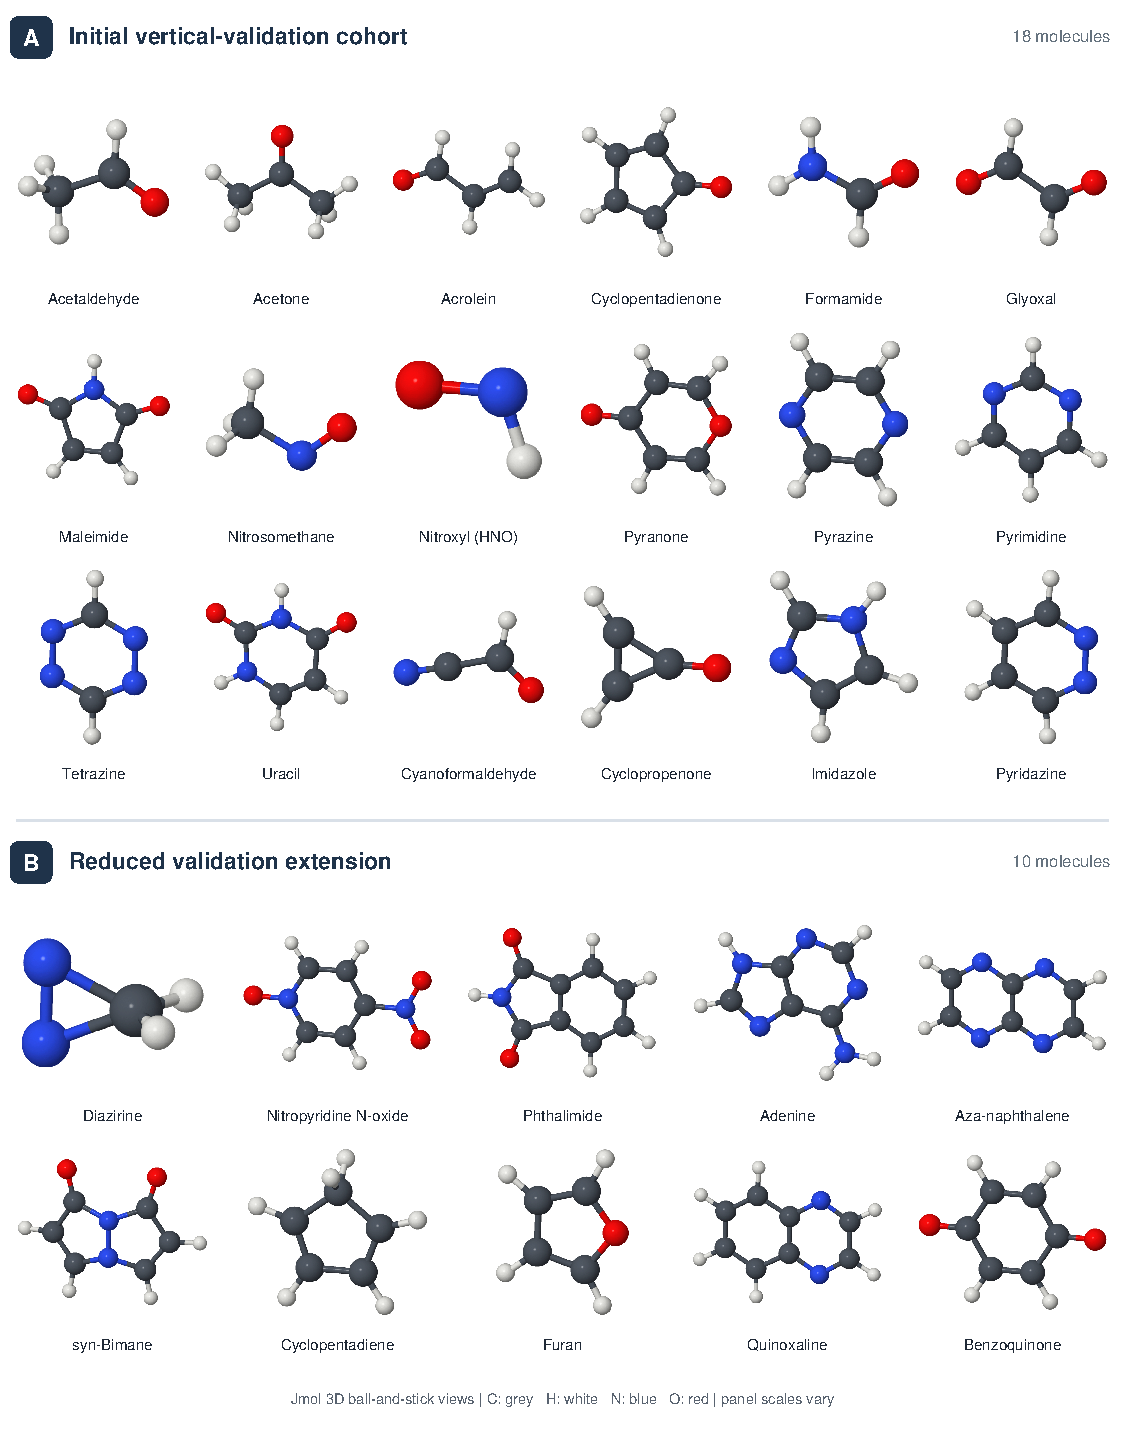
\includegraphics[page=1,width=\linewidth,height=.86\textheight,keepaspectratio]{figures/all_studied_structures_jmol.pdf}\caption{Archived three-dimensional molecular structures, plate 1.}\end{figure}
\begin{figure}[p]\centering\includegraphics[page=2,width=\linewidth,height=.86\textheight,keepaspectratio]{figures/all_studied_structures_jmol.pdf}\caption{Archived three-dimensional molecular structures, plate 2.}\end{figure}
\clearpage
\bibliographystyle{unsrtnat}
\bibliography{references}
\end{document}
